\documentclass[a4paper, 11pt]{article}
\usepackage[margin=0.5in]{geometry}
\usepackage{framed}
\usepackage[brazil]{babel}
\usepackage{graphicx}
\usepackage{xcolor}
\usepackage{verbatim}
\usepackage{blindtext}
\usepackage{xcolor}
% \usepackage{mdframed}
\usepackage{indentfirst}
\usepackage{hyperref}
% \usepackage{txfonts}
\usepackage{amsmath}
\usepackage{titling}
\usepackage{titlesec}

\definecolor{LightGray}{gray}{0.97}
\usepackage{minted}

\usepackage{xcolor} % to access the named colour LightGray

\setminted[fortran]{  framesep=2mm,
  baselinestretch=1.2,
  bgcolor=LightGray,
  fontsize=\footnotesize,
  linenos}

\titleformat{\section}{\normalfont\Large\bfseries}{\thesection}{1em}{}[\titlerule] 
\titleformat{\subsection}{\normalfont\large\bfseries}{\thesubsection}{1em}{} 
% \renewcommand\thesubsection{\Alph{subsection}}
\graphicspath{ {./graficos/} }

\begin{document}
\noindent
\large\textbf{Autor:} Jefter Santiago \hfill \textbf{Projeto 2: {\color{blue}\emph{Equações de ondas - I}}}   \\
\#USP: 12559016 \\
\normalsize Curso: Física Estatística Computacional \\
Prof. F. C. Alcaraz \hfill Data de entrega: 06/04/2024\\
\noindent\rule{7in}{2.8pt}

% \begin{abstract}
% \end{abstract}


\section{Discretização da Equação de Onda}
Nesse trabalhamo buscamos estudar a equação do onda em 1D, para isso partimos da equação
(\ref{eq:eq_onda}) e fazemos a sua discretização. Escolhemos utilizar a discretização para derivadas
simétricas, e portanto obtemos a forma da equação de ondas com a qual trabalharemos (\ref{eq:ondas_discreta})
\begin{equation}
  \frac{\partial^2 \mathcal{Y}}{\partial t^2} = c^2  \frac{\partial^2 \mathcal{Y}}{\partial x^2}
  \label{eq:eq_onda}
\end{equation}

Partindo das derivadas segundas, com \( x = i \Delta x \) e \( t = n \Delta t \) para \( i, n = 1, 2, ... \)  temos
\[  \frac{\mathcal{Y}(i, n+1) + \mathcal{Y}(i,n-1) - 2 \mathcal{Y}(i,n)}{(\Delta t)^2} = c^2 \frac{\mathcal{Y}(i+1,n) + \mathcal{Y}(i-1,n) -
    2\mathcal{Y}(i,n)}{(\Delta x)^2} \]

\[ \mathcal{Y}(i, n+1) + \mathcal{Y}(i,n-1) - 2 \mathcal{Y}(i,n) = \frac{c^2 (\Delta t)^2}{(\Delta x)^2} \left[ \mathcal{Y}(i+1, n) + \mathcal{Y}(i-1,n) - 2\mathcal{Y}(i,n) \right]  \]

fazendo  \( r \equiv  c \Delta t/\Delta x\) podemos escrever as iterações no tempo para cada posição da propagação
na equação abaixo

\begin{equation}
  \mathcal{Y}(i, n+1) = 2 \left( 1 - r^2 \right) \mathcal{Y}(i, n) + r^2 \left( \mathcal{Y}(i+1,n) + \mathcal{Y}(i-1,n) \right) - \mathcal{Y}(i,n-1)
  + \mathcal{O}(\Delta x^2) + \mathcal{O}()
  \label{eq:ondas_discreta}
\end{equation}


Fica claro pela equação (\ref{eq:ondas_discreta}) que para nossa simulação podemos trabalhar com 
vetores que descrevem o estado de uma posição em cada posição, ``anterior'', ``atual'' e
``posterior''. No código das simulações foi implementado uma matrix ``grid'' que computa esses
estados de acordo com a iteração.  

Para finalizar a descrição do problema de propagação de ondas precisamos das condições de
contorno. Nesse projeto inicial foram feitas simulações em condições para propagação ideal de ondas
presas em uma caixa, ou seja, nas extremidades do nosso espaço vale que $\mathcal{Y}(0) = \mathcal{Y}(L) = 0$, para um
comprimento $L$ qualquer e $d \mathcal{Y}(x, t = 0)/ dt = 0$. 


\subsection{Instabilidade numérica}
A escolha dos menores \( \Delta x \) e \( \Delta t \) em geral levam a execuções mais estáveis. Porém, quando
trabalhamos com dois passos diferentes surgem algumas possíveis instabilidades. Buscando simplificar
essas análises escrevemos o fator $r$

\begin{equation}
  r = \frac{\Delta t}{\Delta x} c
  \label{eq:fator_r}
\end{equation}

a partir dessa relação podemos tirar algumas conclusões: \( \Delta x \) e \( \Delta t \) devem variar juntos,
pois se mantermos um deles fixo e variando o outro obtemos uma divergência, por exemplo se \( \Delta x \)
são valores cada vez menores para um \( \Delta t \) fixo e o caso mais estável que podemos obter é no
qual \( r = 1  \).

No projeto iniciamos as simulações no caso mais estável de uma onda ideal com \( r = 1 \) e depois
as situações em que as instabilidades numéricas surgem. Nesses casos foi necessário trabalhar com
menos interações já que os valores de $Y$ divergem muito rapidamente. Então basta algumas iterações
para demonstrarmos esta instabilidade.


Utilizamos valores fixos de \( \Delta x \), escolhidos com base no que funciona melhor para cálculo de
derivadas, vistas na disciplina de \emph{Introdução à Física Computacional}. Com isso
estimamos os valores de \( \Delta t \) para que o \( r \) seja o nosso parâmetro de estabilidade do das simulações.


\subsection{Erro associado à simulação}


\section{Simulações de ondas ideais}


Como foi discutido anteriormente(\ref{})\footnote{Marcar aqui a sessão/subsessão.} o $\Delta x$ escolhido
foi fixado para todas simulações. Além disso a velocidade de nossas ondas também é mantida constante
igual à \( c = 300\) (m/s)  . Com isso podemos variar os paramêtros de \( r \) e \( \Delta t \). 

Foi escolhido um periodo total\footnote{periodo?} de \( t = 0,01\)(s)  de forma que, para uma onda à velocidade da luz
dentro de uma caixa de \( 1\)(m) hajam 3 reflexões.


Foram utilizadas as mesmas rotinas para implementação da simulação com uma única mudança, as
condições iniciais, já que as condições de contorno, isto é, a corda presa nas extremidades, é
válida para simulação das ondas na corda de um violão. Para a simulação de ondas Gaussianas usamos o
modelo de condição inicial dado por 

\begin{equation}
    \mathcal{Y}(x, 0) = \mathcal{Y}_0 (x) = \exp{\left[- \frac{(x-x_0)^2}{\sigma^2}\right]}, x_0 = L/3, \sigma = L/30 \\
  \label{eq:y_0}
\end{equation}
\( d \mathcal{Y} / d t |_{t = 0} = 0 \)
onde no código foi denotado por  \verb|Y0(x,s)|.


Segue abaixo abaixo a estrutura central do programa de simulação de ondas:

\begin{minted}{fortran}[!]
 !     Simulação para ondas ideias
      implicit real*8(a-h, o-y)

!     Grid de estados da computacao:
!     1 -> Anterior
!     2 -> Atual
!     3 -> Proximo
      dimension grid(100, 3)

      ! L 
      s = 1.0d0
      c = 300.0d0

      r = 1.0d0
      nx = 100

      dx = s / (nx*1.d0)

      dt = r * dx / c
      t = 0.01
      nt = floor(t/dt)

      print *, "dx = ", dx
      print *, "dt = ", dt
      print *, "nT = ", nt

      open(unit = 1, file = "saida-tarefa1-a.dat")

      grid(:, 3) = 0.e0
!     aplica as condicoes iniciais ao grid
!     t = 0
      do i = 1, nx
         grid(i, 2) = Y0(i*dx, s)
      end do
!     
      grid(:,1) = grid(:, 2)
      call write_to_file(grid, nx)
!     t = 1
      grid(:, 2) = grid(:, 1)
!     simulação
      do n = 3, nt
         call drive_pulse(grid, nx, r)
         call write_to_file(grid, nx)
      end do
      close(1)
      end 

      subroutine write_to_file(grid, nx)
      implicit real*8(a-h, o-y)
      dimension grid(100, 3)
      write(1, '(3000F16.8)') (grid(i, 2), i=1, nx)
      end subroutine write_to_file

      subroutine drive_pulse(grid, nx, r)
      implicit real*8(a-h, o-y)
      dimension grid(100, 3)
!     y_next = 2(1-r^2)y_curr + r^2[y(t+1,n)+y(t-1,n)] - y_prev
      grid(1, 3) = grid(1, 2)
      grid(nx,3) = grid(nx, 2)

      y = 2.e0*(1.e0-r*r)

      do i = 2, nx-1
         grid(i,3)=y*grid(i,2)+r*r*(grid(i+1,2)+grid(i-1,2))-grid(i,1)
      end do
!     swap
      grid(:, 1) = grid(:, 2)
      grid(:, 2) = grid(:, 3)
      end subroutine drive_pulse      
\end{minted}
\footnote{Trazer uma discussão sobre escolhas de implementação -> por exemplo uso do grid.}


Para o programa as simulações de ondas em uma corda temos a condição inicial dada por
(\ref{eq:y_0}), implementada por

\begin{minted}{fortran}[!]
      function Y0(x, s)
      implicit real*8(a-h, o-y)
      Y0 = exp(-((x-
    \item s/3)**2)/(s/30)**2)
      end
\end{minted}

condição aplicada à todo o grid na linhas linhas $32$ à $34$\footnote{Ficar de olho se isso n vai mudar...} do programa.

\clearpage
\subsection{Caso de \( r = 1 \) }

Como podemos ver na figura (\ref{fig:tarefa1-a}) a oscilação não apresenta nenhuma deformação, e
fazendo valores maiores de \( t \) e observando o comportamento da onda não surgem deformações para
\( r = 1 \). Para condição de contorno de bordas fixas é esperado que a onda seja espelhada nas
reflexões, e é o que observamos para os dois pacotes à esquerda e à direita. A primeira reflexão
acontece em torno da iteração 30  e a segunda na iteração 70.

Ocorrem interferências de forma construtiva, pois pelas condições impostas ambos se encontram sempre
do mesmo lado da reflexão e se somam formando a amplitude completa inicial.
A configuração inicial do sistema vai se repetir na iteração número $200$, isto é, no tempo
\( 200 \cdot \Delta t \). Como nosso \( \Delta t\) utilizado é dado pela (\ref{eq:fator_r}), então \( \Delta t = 1 \cdot
\Delta x / 300  \approx 3 \cdot 10^{-5} \) será a configuração inicial se repete em \( t = 0,006 \) (s). Esse
é o tempo necessário para cada um dos pacotes menores percorrerem \( 2 L\). Para um \( L \)
qualquer, temos então \( t = 2 L / c \) será o tempo em que a situação inicial surge novamente.


\begin{figure}[h!] 
    \centering
    \centering
    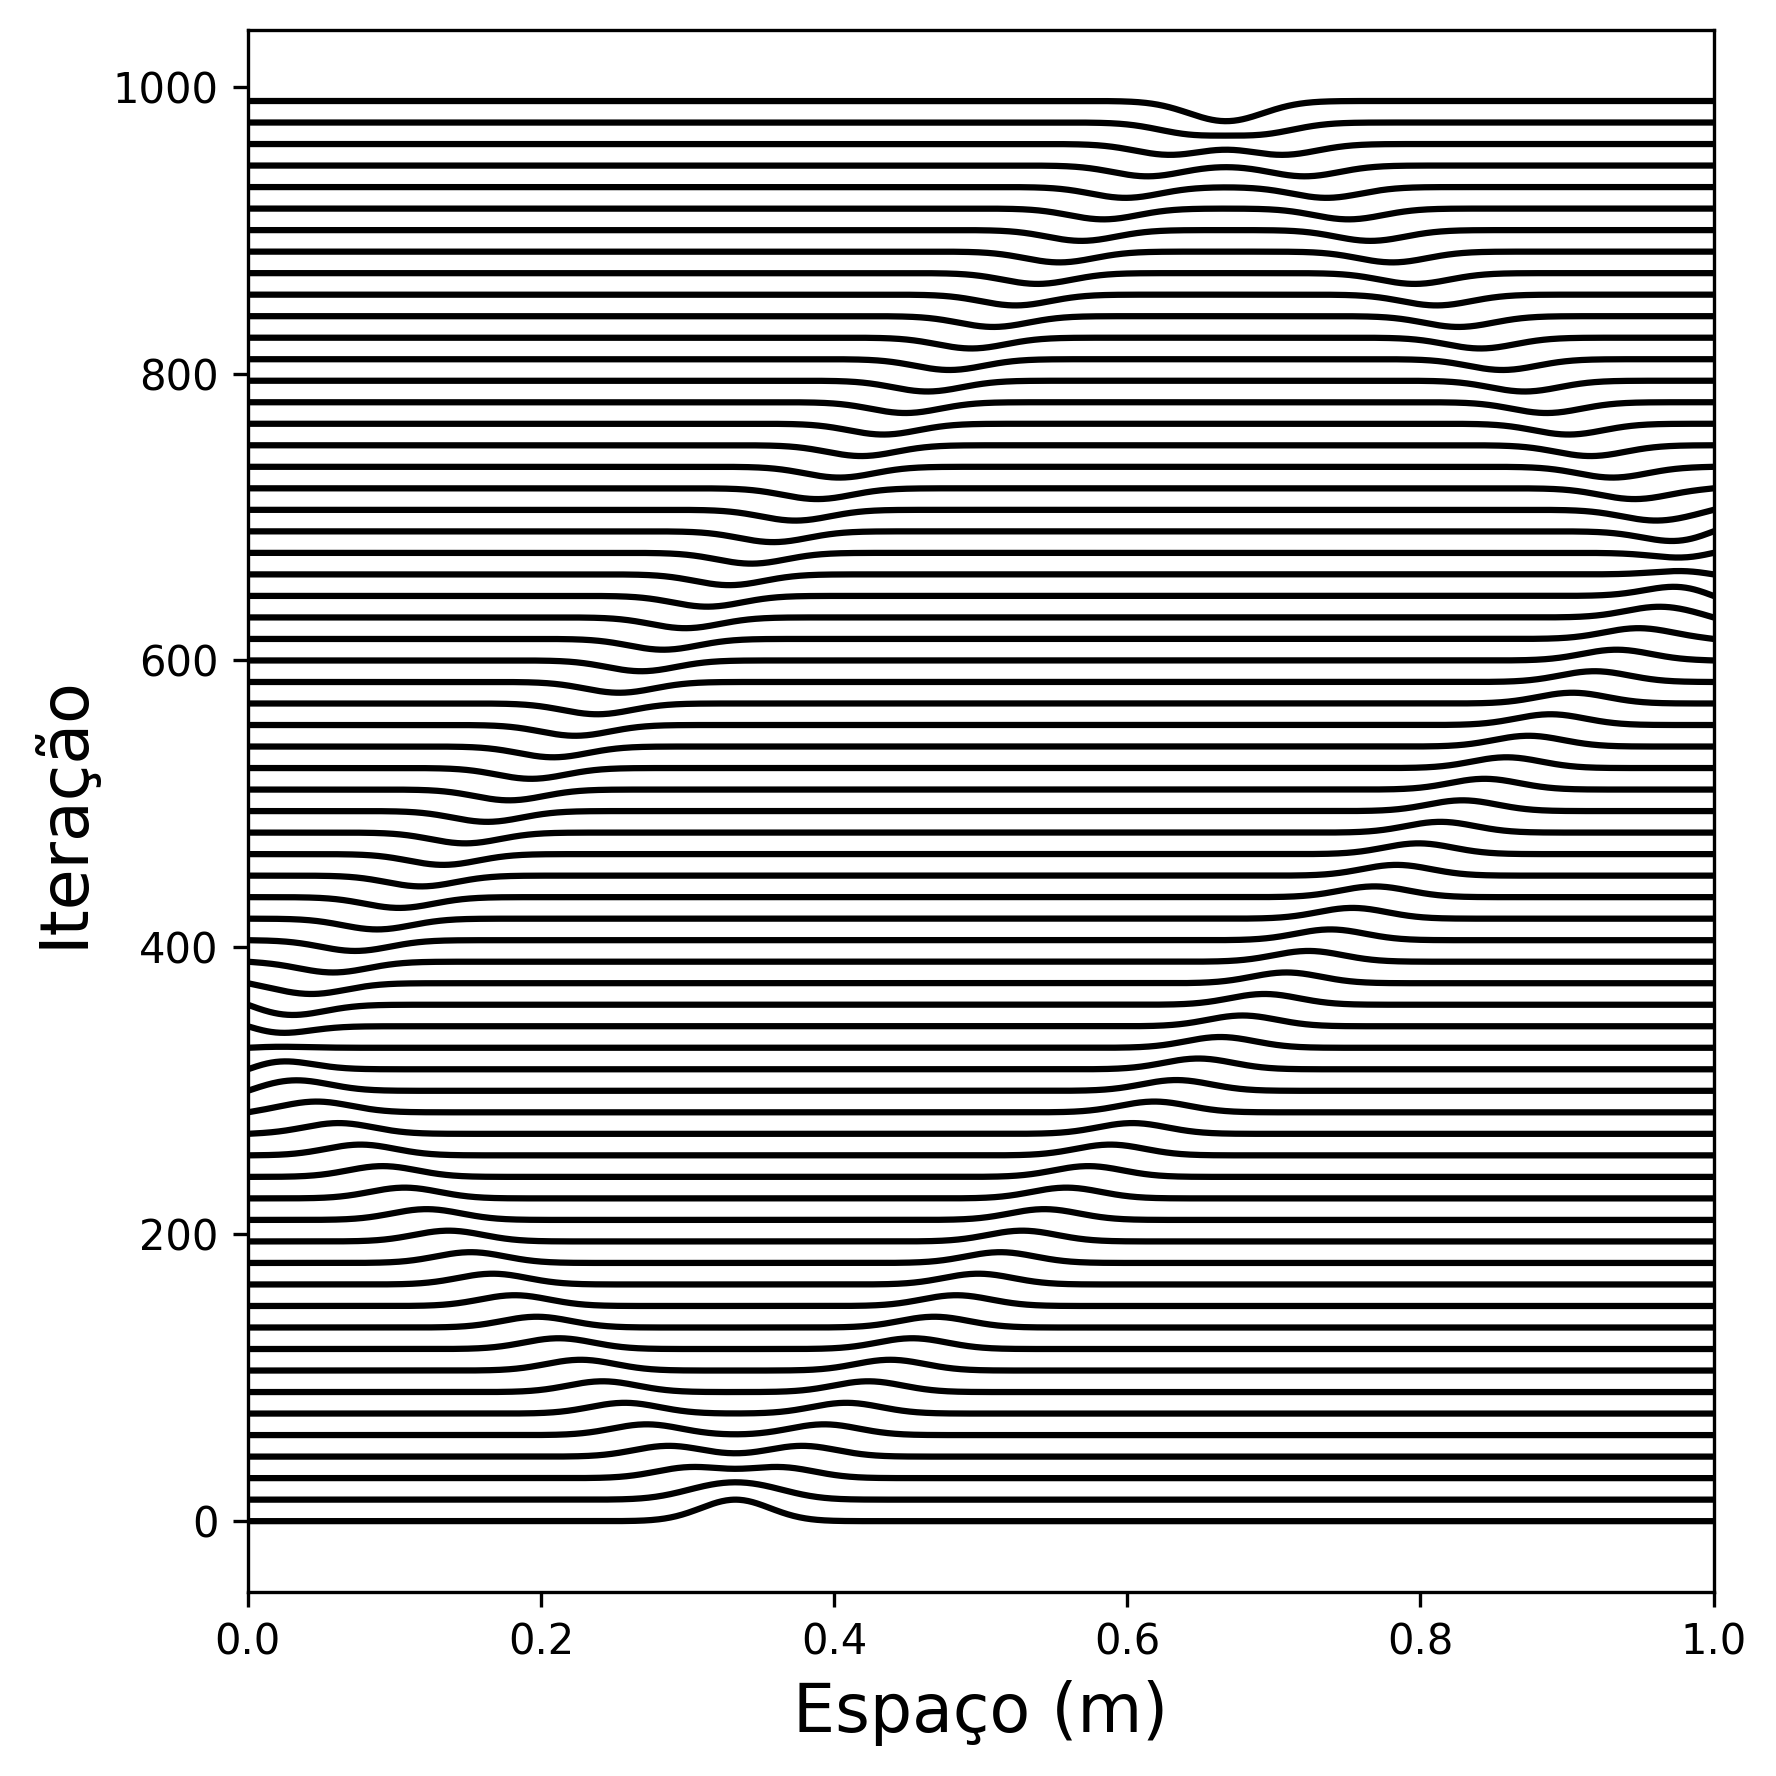
\includegraphics[width=0.45\textwidth]{graf-tarefa1-a}
    \caption{Evolução temporal da onda em para $100$ iterações. Apenas metade dessas iterações estão
      estão nessa figura para melhor visualização das frentes de ondas.}
    \label{fig:tarefa1-a}
\end{figure}

\clearpage
\subsection{Caso de \( r = 2 \) }


Nesse caso podemos observar a instabilidade desse que surge para valores de \( r > 1  \).
A amplitude das ondas diverge muito rápido e na simulação bastaram pouquissímas iterações
para que visualizarmos o comportamento anômalo \footnote{boa palavra?} da onda.

O algoritmo diverge para \( r > 1 \) pois \footnote{Explicar pq explode}

\begin{figure}[h!] 
    \centering
    \centering
    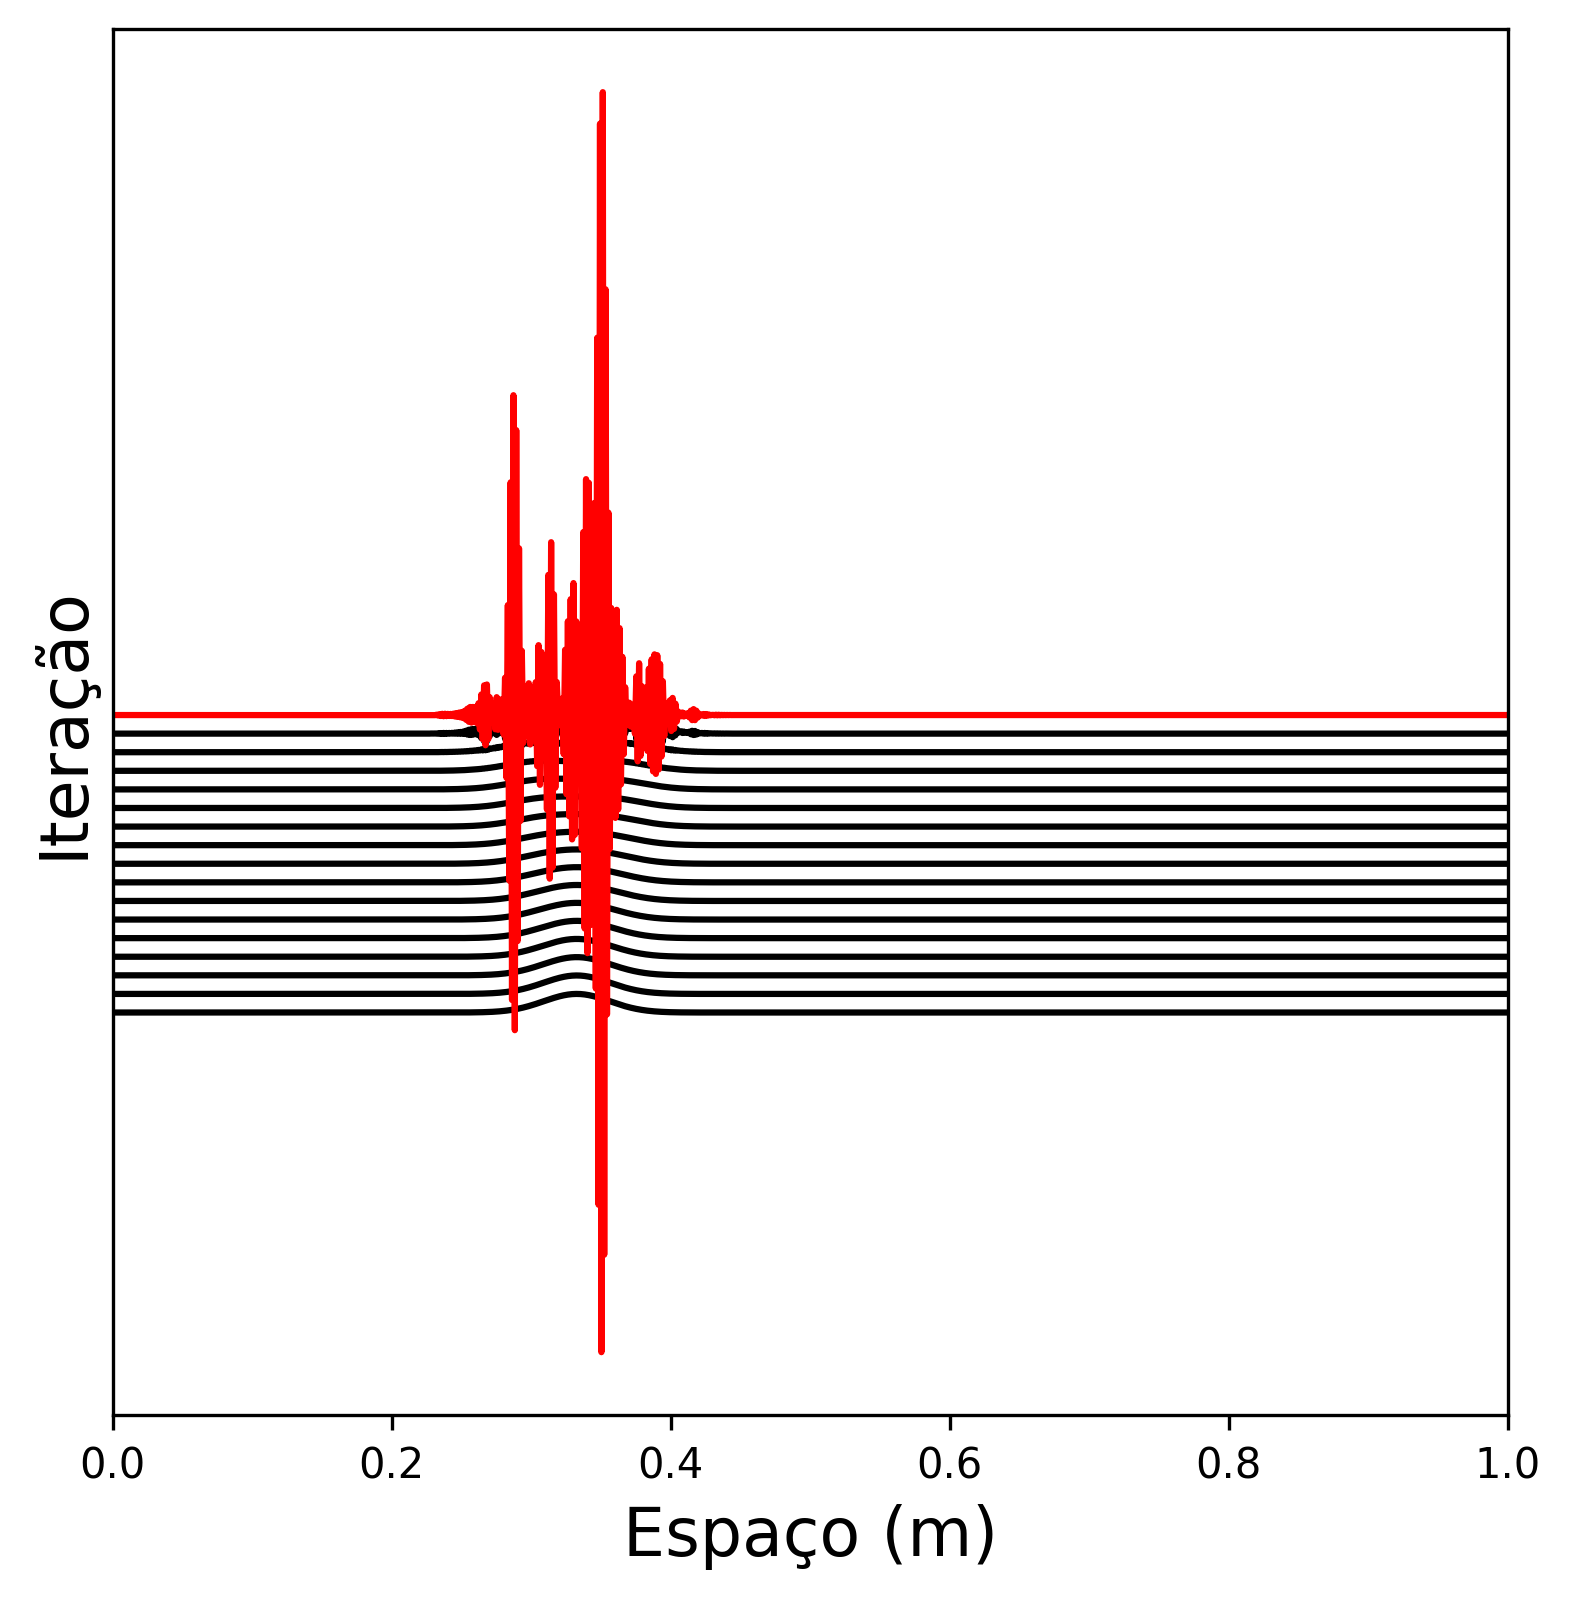
\includegraphics[width=0.4\textwidth]{graf-tarefa1-b}
    \caption{}
    \label{fig:tarefa1-b}
\end{figure}

\subsection{Caso de \( r = 0.25 \) }

A implementação com valores de \( r < 1 \) apresentam certa estabilidade, porém para tempos
grandes é possível observar deformações no pacote gaussiano. E além disso, para tempos pequenos
apesar de simular bem, não é eficiente computacionalmente, já que executa muito mais iterações. Isso porque, para
\( \Delta x \), \( c \) e \( r \) fixos, precisamos alterar o parâmetro de \( \Delta t \), o que aumenta
o número de iterações do nosso programa.

\begin{figure}[h!] 
    \centering
    \caption{Simulação para \( r = 0,25 \) nas primeiras iterações.}
    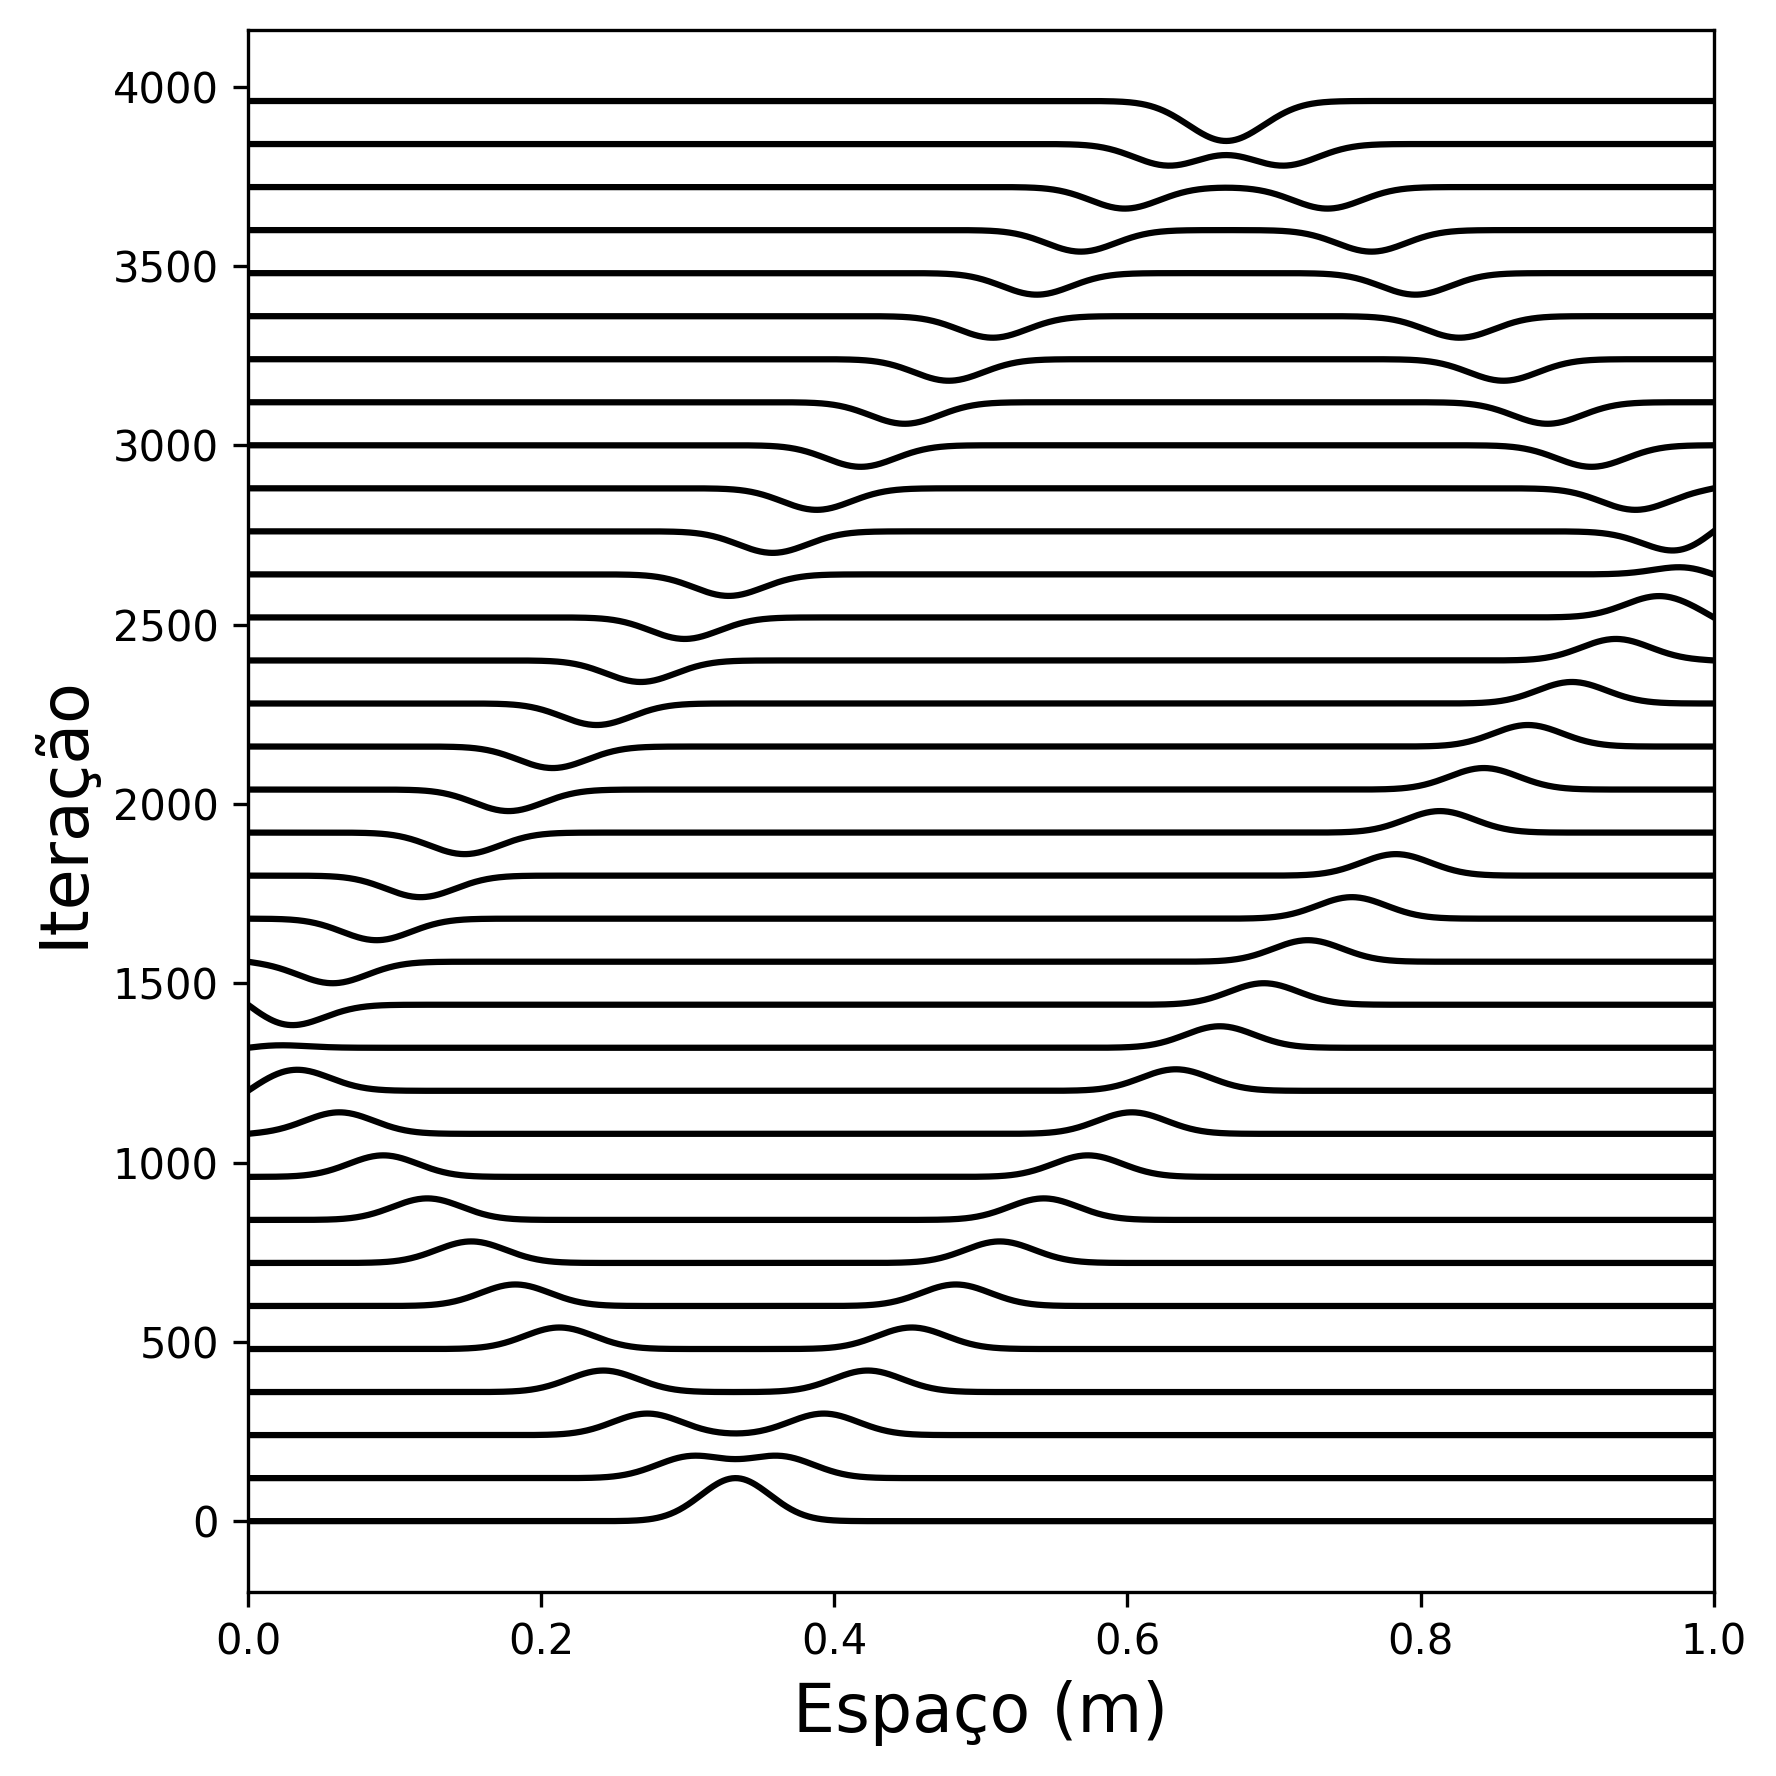
\includegraphics[width=0.4\textwidth]{graf-tarefa1-c1}
    \label{fig:tarefa1-c1}
\end{figure}


A figura (\ref{fig:tarefa1-c}) foi construída a partir da simulação com \( r = 0.25 \) e \( t = 0,02
\). No gráfico temos o comportamento da onda para um tempo grande, após muita iterações e podemos
ver claramente as deformações do pacote gaussiano.

\footnote{Falar sobre o número de iterações ser bem maior partindo da expressão do (\ref{eq:fator_r})}
\begin{figure}[h!] 
    \centering
    \caption{Comportamento da onda para um tempo grande.}
    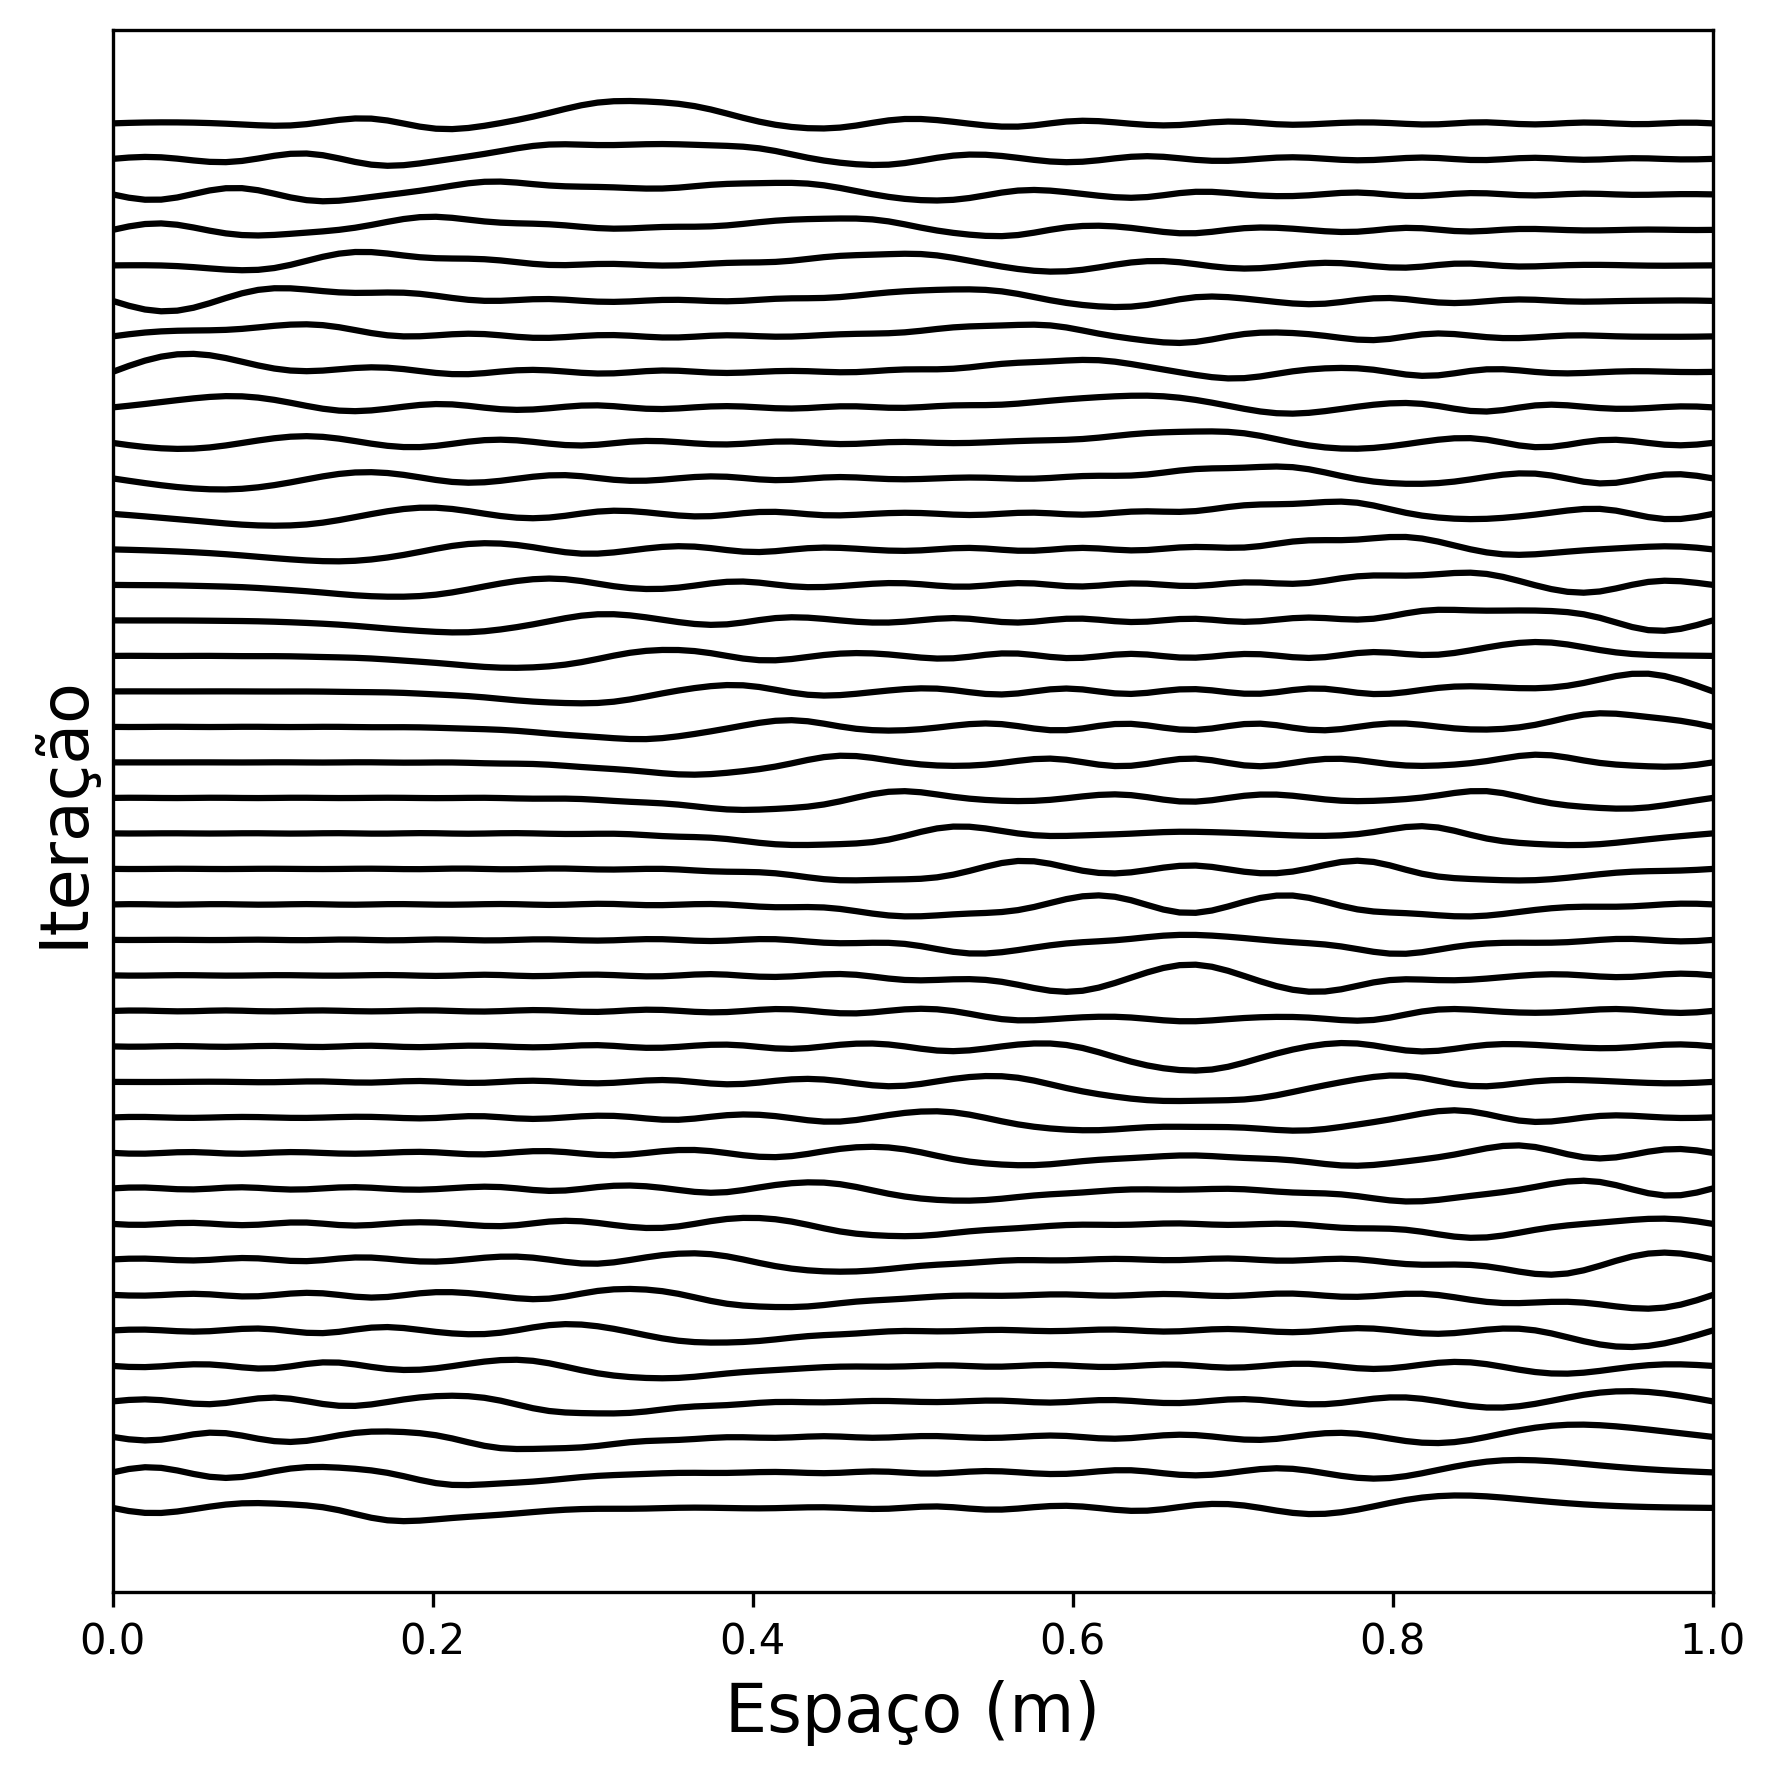
\includegraphics[width=0.4\textwidth]{graf-tarefa1-c}
    \label{fig:tarefa1-c2}
\end{figure}

\section{Simulação de ondas na corda de violão}

Já o perfil inicial de pinça, na corda do violão, foi chamado de \verb|Y0_pinca(x, s)|, e pela
figura dada no projeto temos que o perfil inicial da onda deverá ser (\ref{})\footnote{Linkar a sessão que discuto aquilo aqui.}

\begin{equation}
  \mathcal{Y}(x, 0) = \mathcal{Y}_0(x) = \begin{cases}
    x, x < L/4\\
    \frac{1}{3} \left( L - x \right), L/4 \leq x \leq L
  \end{cases}
  \label{eq:y_0_pinca}
\end{equation}



\subsection{Caso de \( r = 1 \) }

\begin{figure}[h!] 
    \centering
    \centering
    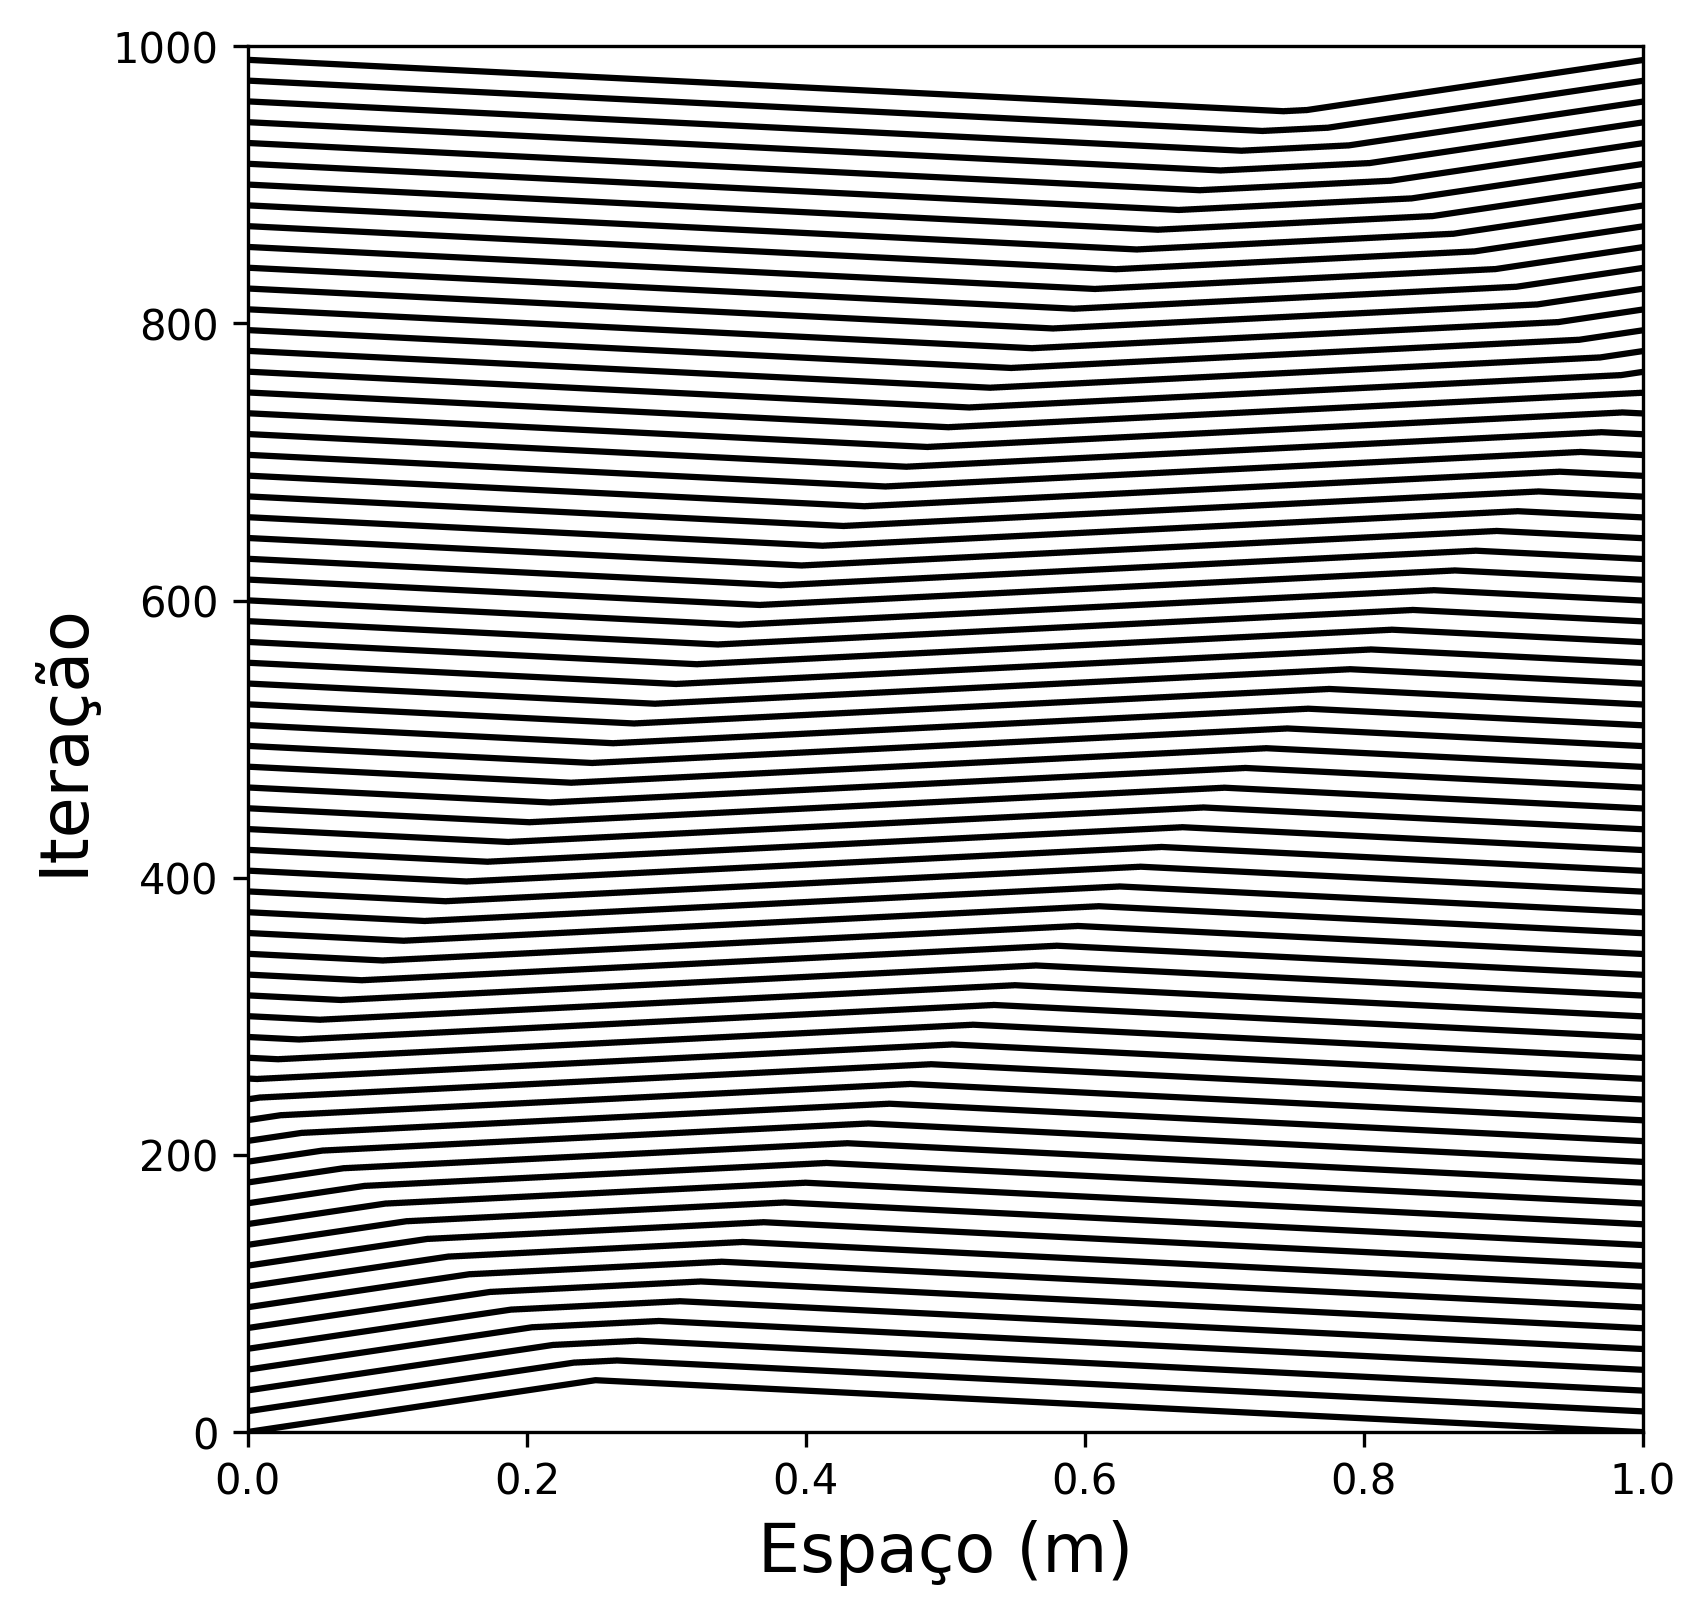
\includegraphics[width=0.4\textwidth]{graf-tarefa2-a}
    \caption{}
    \label{fig:subA}
\end{figure}


\subsection{Caso de \( r = 2 \) }


\footnote{Explicar pq explode}
\begin{figure}[h!] 
    \centering
    \centering
    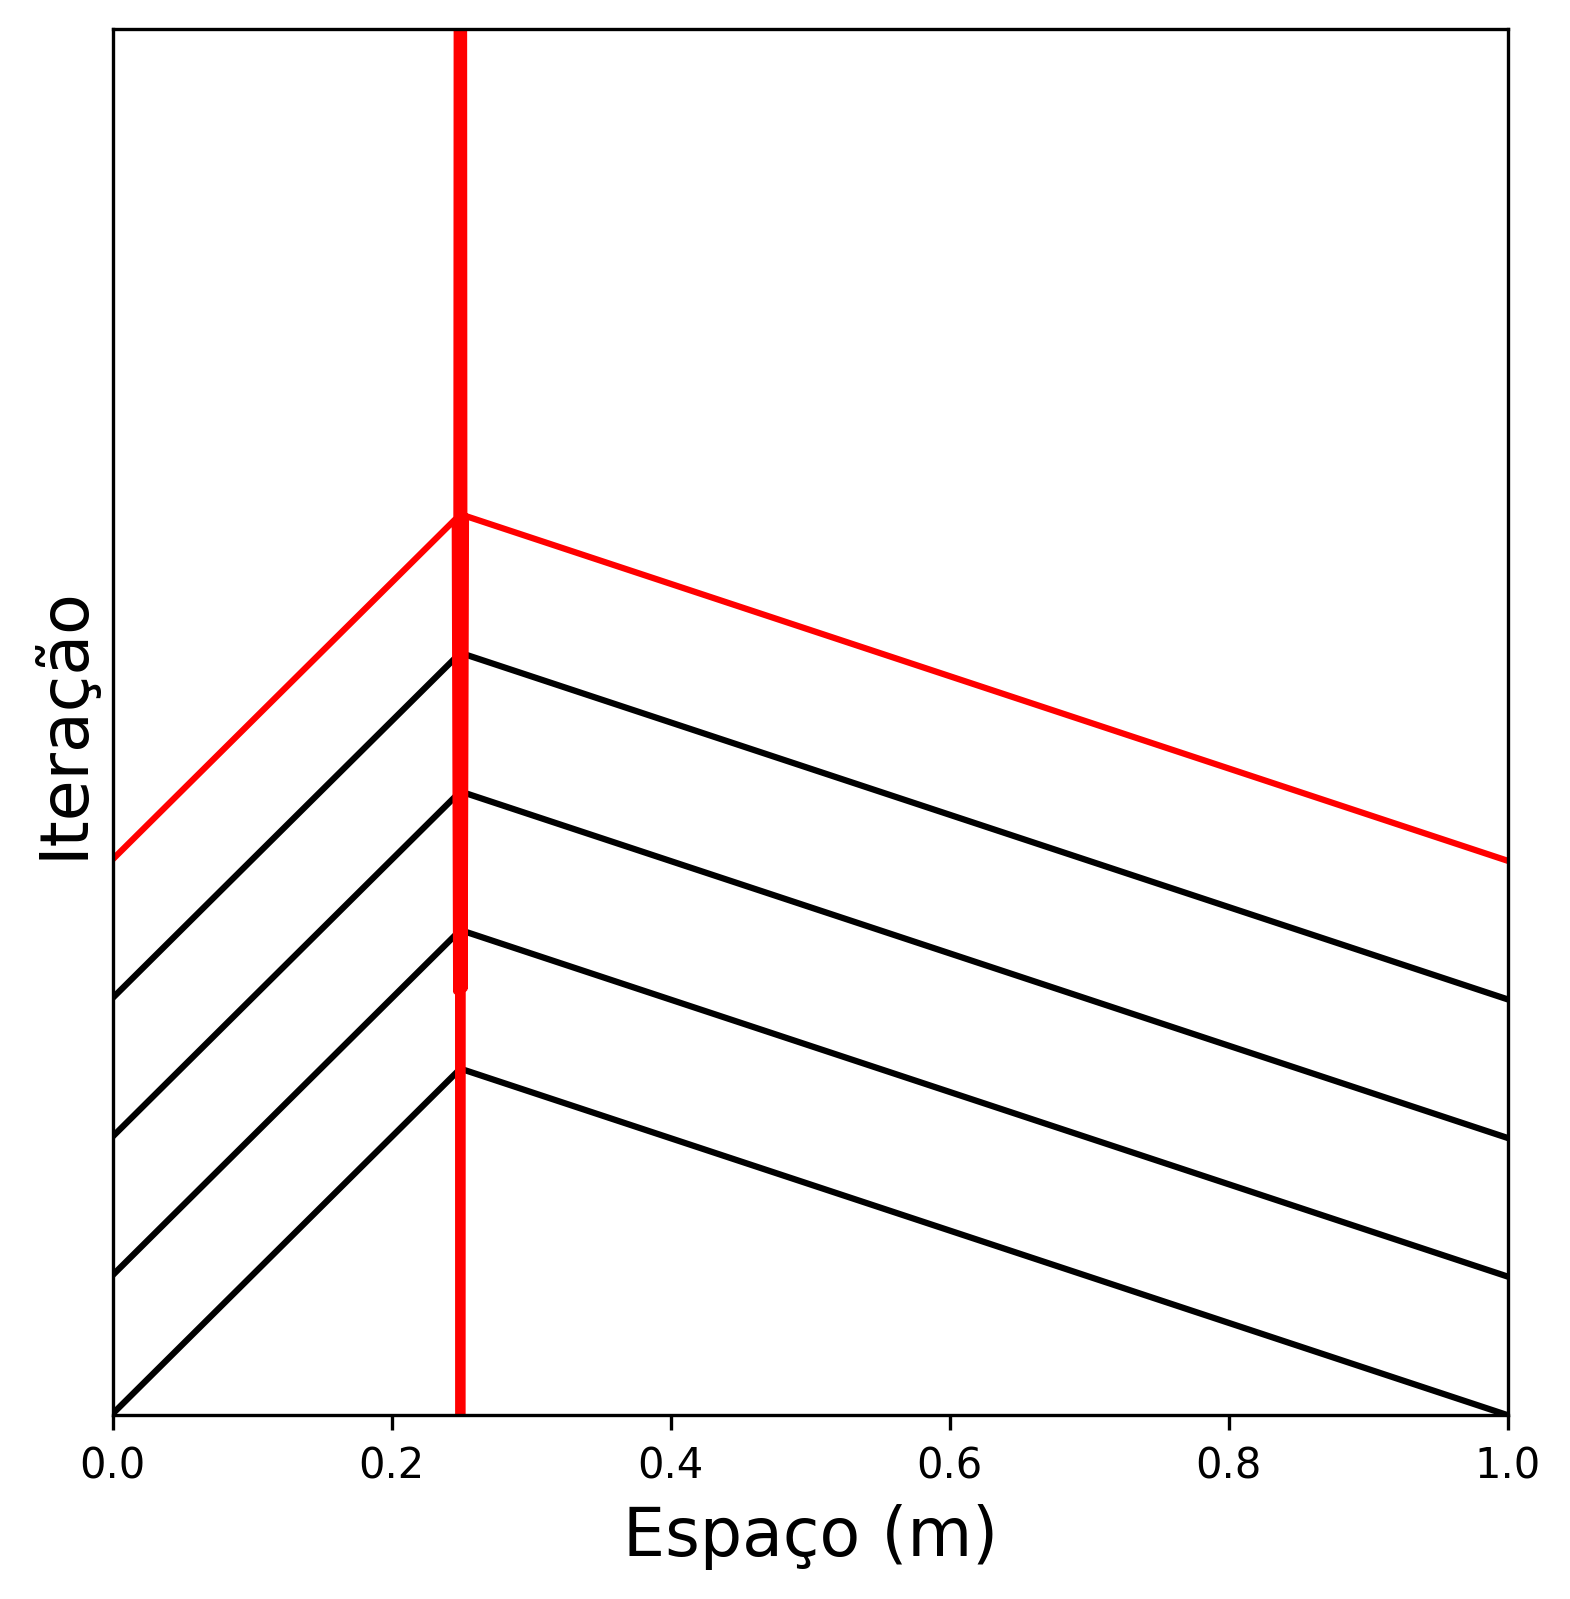
\includegraphics[width=0.4\textwidth]{graf-tarefa2-b}
    \caption{}
    \label{fig:subB}
\end{figure}

\subsection{Caso de \( r = 0.25 \) }



\footnote{Falar sobre o número de iterações ser bem maior partindo da expressão do (\ref{eq:fator_r})}
\begin{figure}[h!] 
    \centering
    \centering
    \includegraphics[width=0.4\textwidth]{graf-tarefa2-c}
    \caption{}
    \label{fig:subC}
\end{figure}

\footnote{Discutir solução analitica do problema da lista de Fismat -> talvez colocar ele no projeto
  e computar a série para comparação.}
\end{document}
%%% Local Variables:
%%% mode: latex
%%% TeX-master: "main.tex"
%%% End:
